\documentclass[dvipsnames, svgnames, x11names]{beamer}
\usetheme{mytheme2024}
\special{dvipdfmx:config z 0} %取消PDF压缩，加快速度，最终版本生成的时候最好把这句话注释掉

\title{化学反应工程}
\subtitle{第四章\ 管式反应器}
\author{张斌}
\institute[理工系]{河北农业大学 理工系}
\date{\the\year 年 \the\month 月}
%-----------------------------------------------------------------
\begin{document}

\maketitle

	\begin{frame}
		\frametitle{管式反应器}
	
		长度远大于其直径的一类反应器，统称管式反应器。
		
		管式反应器可用于均相反应，也可用于多相反应。
		
		管式反应器多数采用连续操作，少数采用半间歇操作，使用间歇操作的极罕见。
		\begin{figure}[h]

			\centering
			
			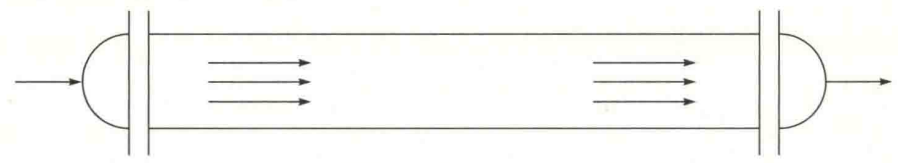
\includegraphics[width=.75\linewidth]{figs/fig4.0.png}
			
		\end{figure}
		很多气相反应在高温下反应速率较快，反应时间短，即使反应物在很短的时间内通过一定温度条件下的管式反应器，也可以得到满意的转化率。对于反应速率较快的液相反应，也可以采用连续流动管式反应器。

		管式反应器比表面积相对釜式反应器较大，传热容易，因此常用于强放热反应，或者强吸热反应。	
	\end{frame}

	\begin{frame}{}
        \begin{center}
            {\Huge \cbf{目 \ 录}}
        \end{center}
		\tableofcontents
		\thispagestyle{empty}
		\addtocounter{framenumber}{-1}
	\end{frame}




    \section{理想流动模型}


    \begin{frame}
        \frametitle{流动模型}
        流体在连续反应器中的流动是一种极其复杂的物理现象，而这种现象又直接影响到器内化学反应进行的速率和程度。
        
        流体在管内的径向流速分布是不均匀的，以中心处的流速最大，靠壁处最小。
        \begin{columns}[c]
            \column{5cm}
                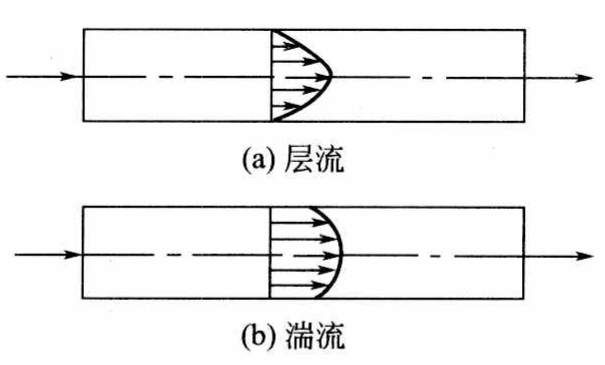
\includegraphics[width=\linewidth]{figs/fig4.1ab.png}
            \column{8.5cm}
                (a) 当流速很小时，流体分层流动，互不混合，称为层流，其径向流速分布为抛物面状；
        
                (b) 当流速增加到很大时，呈湍流，随湍动的程度不同流速分布变得扁平。
        \end{columns}
        显然，中心部分的流体停留时间短，靠近管壁处的流体停留时间则长。停留时间不同，反应程度自然就不一样。
    
        除了流速分布外，器内的流体混合也是一个极其重要因素。因为流体混合的形式和程度直接影响到器内各处流体的浓度和温度。
    
    \end{frame}
    
    
    \begin{frame}
        \frametitle{活塞流模型}
        \begin{figure}[h]
    
            \centering
            
            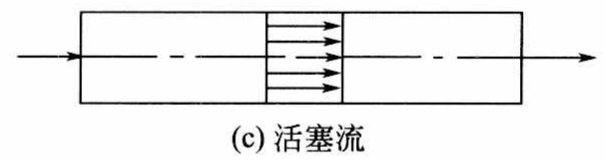
\includegraphics[width=.6\linewidth]{figs/fig4.1c.png}
            
        \end{figure}
        活塞流模型是最基本的一种流动模型。其基本假定如下：    
        \begin{columns}[c]
            \column{0cm}         
            \column{13.5cm}
            \begin{itemize}
                \item[假定1] 径向流速分布均匀；
                \item[假定2] 在垂直于流体流动方向的任何横截面上，浓度均匀，温度均匀，即径向混合均匀；
                \item[假定3] 流体流动方向即轴向上不存在流体的混合，即不存在返混。
                \item[假定4] 由于流体的主体流动和发生化学反应的结果，各个横截面上反应物料的浓度和温度可以是各不相同的。
            \end{itemize}    
        \end{columns}
    \end{frame}
    
    
    \begin{frame}
        \frametitle{全混流模型}
    
        \large 连续釜式反应器是另一种流动模型，这种流动模型叫做完全混合流模型，简称全混流模型。
    
        其基本假定是无论径向混合还是轴向混合都达到最大。最大的径向混合和轴向混合保证了整个反应器内反应物料的浓度均一、温度均一。
        
        活塞流和全混流的根本差别是，前者无返混存在，后者的返混程度则达到最大。
    
        活塞流和全混流都属于理想化了的流动，所以这两种模型又称为理想流动模型。
    
    \end{frame}



\section{等温管式反应器设计}


\begin{frame}
    \frametitle{活塞流模型管式反应器的设计方程}
    \begin{columns}[c]
        \column{2.6cm}
            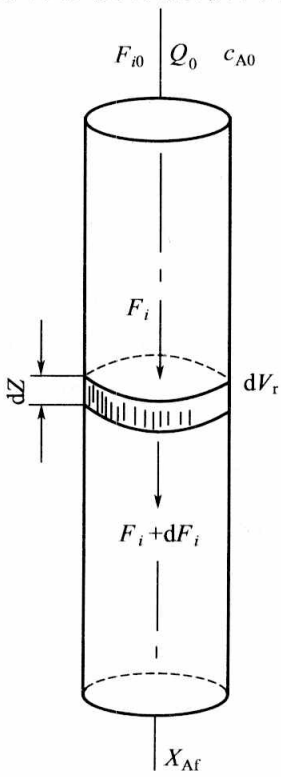
\includegraphics[width=\linewidth]{figs/fig4.2.png}
        \column{10.9cm}
            取微元体积$\mathrm{d}V_\mathrm{r}$作为控制体积，对此微元体作任意反应组分$i$的物料衡算，当过程达到定态时，
            \[
                F_{i}+\mathrm{d} F_{i}-F_{i}=\mathscr{R}_{i} d V_{\mathrm{r}}
            \]
            \[
                \mathrm{d} F_{i} = \mathscr{R}_{i} d V_{\mathrm{r}}
            \]
            \[
                \frac{\mathrm{d} F_{i}}{d V_{\mathrm{r}}}=\mathscr{R}_{i}
            \]
    \end{columns}
\end{frame}


\begin{frame}
    \frametitle{物料衡算式}

    对于单一反应，只要对一个反应组分即关键组分作物料衡算就够了。
    \[
        \frac{\mathrm{d} F_{\mathrm{A}}}{d V_{\mathrm{r}}}=\mathscr{R}_{A}
    \]
    为计算反应体积，将$F_{\mathrm{A}}$与$\mathscr{R}_{A}$变为转化率的函数较为方便。
    
    将$F_{\mathrm{A}}=F_{\mathrm{A0}}(1-X_{\mathrm{A}})$代入，得
    \[
        F_{\mathrm{A} 0} \frac{\mathrm{d} X_{\mathrm{A}}}{\mathrm{d} V_{\mathrm{r}}}=-\mathscr{R}_{\mathrm{A}}
    \]
    因$F_{\mathrm{A0}}=Q_0 c_{\mathrm{A0}}$，上式又可写成
    \[
        Q_0 c_{\mathrm{A0}} \frac{\mathrm{d} X_{\mathrm{A}}}{\mathrm{d} V_{\mathrm{r}}}=-\mathscr{R}_{\mathrm{A}}
    \]
    以上均为管式反应器的设计方程，实际应用时可根据具体情况选定。

\end{frame}


\begin{frame}
    \frametitle{反应体积的计算}
    \[
        \mathrm{d} V_{\mathrm{r}} = Q_0 c_{\mathrm{A0}} \frac{\mathrm{d} X_{\mathrm{A}}}{-\mathscr{R}_{\mathrm{A}}}
    \]
    积分管式反应器设计方程可得反应体积
    \[
        V_{\mathrm{r}}=Q_{0} c_{\mathrm{A} 0} \int_{0}^{X_{\mathrm{Af}}} \frac{\mathrm{d} X_{\mathrm{A}}}{-\mathscr{R}_{\mathrm{A}}}
    \]
    \[
        \tau = \frac{V_{\mathrm{r}}}{Q_{0}} = c_{\mathrm{A} 0} \int_{0}^{X_{\mathrm{Af}}} \frac{\mathrm{d} X_{\mathrm{A}}}{-\mathscr{R}_{\mathrm{A}}} 
    \]
    间歇釜式反应器的反应时间：
        \[
            t=c_{\mathrm{A} 0} \int_{0}^{X_{\mathrm{Af}}} \frac{\mathrm{d} X_{\mathrm{A}}}{-\mathscr{R}_{\mathrm{A}}}
        \]
        \begin{alertblock}{}
            等容下反应，$\tau=t$；变容下反应，$\tau \neq t$
        \end{alertblock}
\end{frame}


\begin{frame}
    \frametitle{什么情况下管式反应器是非恒容的？}
    当反应过程中流体的\bf{体积流量}发生变化时，就是非恒容的。这主要发生在：
    \begin{enumerate}
      \item 总摩尔数发生变化的气相反应（最常见）
      \item 反应过程中有显著的压力降
      
      即使是总摩尔数不变的气相反应，如果反应器很长或流速很快，导致从入口到出口压力显著降低，根据 $pV=nRT$，在恒温下，压力$p$的下降会导致体积$V$的膨胀，体积流量也会增加。这同样是非恒容行为。
      \item 温度发生显著变化的反应
      
      如果反应器不是等温的（例如绝热反应器或伴有强放/吸热的反应），温度$T$的变化会直接导致体积$V$的变化（热胀冷缩），从而改变体积流量。
    \end{enumerate}
    \begin{alertblock}{}
        管式反应器并非都是恒容的。在处理气相反应时，必须首先检查其总摩尔数在反应前后是否发生变化，以确定是否需要使用非恒容模型进行分析和设计。
    \end{alertblock}
\end{frame}


\begin{frame}
    \frametitle{反应以等速率进行的情况}
    \[
        V_{\mathrm{r}}=Q_{0} c_{\mathrm{A} 0} \int_{0}^{X_{\mathrm{Af}}} \frac{\mathrm{d} X_{\mathrm{A}}}{-\mathscr{R}_{\mathrm{A}}}
    \]
    如果反应系以等速率进行，则$\mathscr{R}_{\mathrm{A}}$为常数，上式可化为
    \[
        V_{\mathrm{r}}=\frac{Q_{0} c_{\mathrm{A} 0} X_{\mathrm{Af}}}{-\mathscr{R}_{\mathrm{A}}(X_{\mathrm{Af}})}
    \]
    此时与连续釜式反应器的反应体积一致：
    \[
        V_{\mathrm{r}}=\frac{Q_{0} c_{\mathrm{A} 0} X_{\mathrm{Af}}}{-\mathscr{R}_{\mathrm{A}}(X_{\mathrm{Af}})}
    \]
    \begin{question}
        什么情况下反应会以等速率进行？
    \end{question}
\end{frame}


\begin{frame}[t]
    \frametitle{}
    \begin{redblock}{思考与讨论}
        在间歇釜式反应器中，反应物系的浓度则随时间而变，与位置无关。
        \[
            \frac{\mathrm{d} c_{\mathrm{A}}}{\mathrm{d} t}=\mathscr{R}_{\mathrm{A}}
        \]
        在连续釜式反应器中，反应物系的浓度既不随时间而变，也不随位置而变。

        在管式反应器中，反应物系的浓度变化情况是怎样的？
        \begin{figure}[htpb]
            \centering
            
\includegraphics[width=.6\linewidth]{管式}
        \end{figure}
    \end{redblock}
\end{frame}


\begin{frame}
    \frametitle{管式反应器的轴向浓度分布}

    设$u_0$为反应器进口处流体的流速，$Q_0 = u_0\cdot S$，$\dif V_\mathrm{r} = S\cdot \dif Z$，
    
    可将$Q_0 c_{\mathrm{A0}} \frac{\mathrm{d} X_{\mathrm{A}}}{\mathrm{d} V_{\mathrm{r}}}=-\mathscr{R}_{\mathrm{A}}$写成转化率与轴向距离$Z$的关系式：
    \[
        u_0 c_{\mathrm{A0}} \frac{\mathrm{d} X_{\mathrm{A}}}{\mathrm{d} Z}=-\mathscr{R}_{\mathrm{A}}
    \]
    若为等容过程，可写成轴向浓度分布方程
    \[
        u_0 \frac{\mathrm{d} c_{\mathrm{A}}}{\mathrm{d} Z}=\mathscr{R}_{\mathrm{A}}
    \]
    对于定态操作的活塞流反应器，反应物系的浓度系随轴向距离而变，与时间无关。

    

\end{frame}


\begin{frame}[t]
    \frametitle{}
    \begin{block}{例：管式反应器反应体积的计算}
        采用活塞流管式反应器，等温下进行某均相反应\ch{A -> B}，$r_\mathrm{A}=5.2c_\mathrm{A}$ (\si{mol.L^{-1}.h^{-1}})，每天生产B 20kmol，A的初始浓度为2mol/L，最终转化率为80\%。计算总反应体积。
    \tcblower
    \vspace{-0.5em}
    \[
        Q_0 = \frac{20000}{24\times 0.8 \times 2} = 520.8 \mathrm{L}
    \]
    \pause
    \only<2>{
        \[
        \tau =\frac{1}{k}\ln \frac{1}{1-X_{\mathrm{A}}}=\frac{1}{5.2}\ln \frac{1}{1-0.8}=0.3095 \mathrm{h}
    \]
    \[
        V_{\mathrm{r}}=Q_{0}\tau = 520.8 \times 0.3095 = 161.2 \mathrm{L}
    \]
    }
    \only<3>{
        \[
            V_{\mathrm{r}}=Q_{0}\tau = 520.8 \times 0.3095 = 161.2 \mathrm{L}
        \]
        \begin{table}
        \begin{tabular}{|c|c|c|c|}
            \hline
            间歇釜 $(t_0=0.25\mathrm{h})$ & 连续釜 & 双釜串联 & 管式反应器\\
            \hline
            292 L & 401 L & 247.6 L & 161.2 L\\
            \hline
        \end{tabular}
    \end{table}
    }
    \end{block}
\end{frame}


\begin{frame}[t]
    \frametitle{}
    \begin{redblock}{习题4.1}
        在常压及800℃等温下在活塞流反应器中进行下列气相均相反应：
        \[
            \ch{C6H5CH3 + H2 -> C6H6 + CH4}
        \]
        在反应条件下该反应的速率方程为：
        \[
            r = 1.5 c_\mathrm{T} c_\mathrm{H}^{0.5} \qquad \si{mol.L^{-1}.s^{-1}}
        \]
        式中$c_\mathrm{T}$及$c_\mathrm{H}$分别为甲苯及氢的浓度，mol/L。原料处理量为 2 kmol/h，其中甲苯与氢的摩尔比等于1。若反应器的直径为50 mm，试计算甲苯最终转化率为 95\%时的反应器长度。
    \end{redblock}
\end{frame}


\begin{frame}[t]
    \frametitle{}
    \begin{block}{例4.2}
        在活塞流反应器中，于923K等温下进行丁烯脱氢反应以生产丁二烯
        \[
            \ch{C4H8 -> C4H6 + H2}
        \]
        反应速率方程为
        \[
            r_\mathrm{A} = kp_\mathrm{A} \quad \si{kmol/(m^3.h)}
        \]
        原料气为丁烯与水蒸气的混合气，丁烯的摩尔分数为10\%。操作压力为$10^5$ Pa。923K时，$k=$\SI{1.079e-4}{kmol/(h.m^2.Pa)}。若要求丁烯的转化率达35\%，空时为多少？
    \end{block}
    \pause
    \begin{question}
        为什么达到同样的转化率，体积增大的变容反应所需空时更大？
    \end{question}
\end{frame}


\begin{frame}
    \frametitle{多个反应}

    当反应器同时进行数个反应时，一个反应变量的变化已不足以描述整个反应过程。与釜式反应器一样，需分别对各关键组分作物料衡算，以获得管式反应器的设计方程组。作法与单一反应的情况完全一样，只是方程数目增加而已。
    \[
        \frac{\mathrm{d} F_{i}}{\mathrm{~d} V_{\mathrm{r}}}=\mathscr{R}_{i} \qquad(i=1,2, \cdots, K)
    \]
    对于等容过程，可选择任何形式的反应变量，但变容过程则以选$F_{i}$作为反应变量较为方便。由于N个反应组分并非都是关键组分，这就需将非关键组分的摩尔流量变为关键组分摩尔流量的函数。

    对于等容过程，应用下两个式子可能要方便些。
    \[
       Q_0\frac{\mathrm{d} c_{i}}{\mathrm{~d} V_{\mathrm{r}}}=\mathscr{R}_{i} \quad \text{或} \quad u_0\frac{\mathrm{d} c_{i}}{\mathrm{~d} Z}=\mathscr{R}_{i} \qquad(i=1,2, \cdots, K)
    \]

\end{frame}


\begin{frame}[t]
    \frametitle{}

    \begin{block}{例4.3}
        气体A$_1$与A$_2$在等温活塞流反应器中等压下进行下列气相反应
        \[\begin{array}{ll}
            2 \mathrm{~A}_{1}+\mathrm{A}_{2} \longrightarrow \mathrm{A}_{3} & \bar{r}_1=k_{1} c_{1}^{2} c_{2} \\
            \mathrm{~A}_{3}+\mathrm{A}_{2} \longrightarrow \mathrm{A}_{4} & \bar{r}_2=k_{2} c_{3} c_{2} \\
            2 \mathrm{~A}_{4} \longrightarrow \mathrm{A}_{5} & \bar{r}_3=k_{3} c_{4}^{2}
            \end{array}
        \]
        以$F_i$及$V_\mathrm{r}$为变量，列出反应器的设计方程。假定进料中不含反应产物。
    \end{block}

\end{frame}


\begin{frame}[t]
    \frametitle{}
    \begin{block}{例4.4}
        在管式反应器中于4.05 MPa 及 936 K 等温下进行三甲基萘脱烷基反应：
        \[
            \begin{aligned}
                \ch{T + H2 -> D + CH4}  \qquad r_1 &= k_1c_\mathrm{T}c_\mathrm{H}^{0.5} \quad \si{kmol.m^{-3}.s^{-1}}\\
                \ch{D + H2 -> M + CH4}  \qquad r_2 &= k_2c_\mathrm{D}c_\mathrm{H}^{0.5} \quad \si{kmol.m^{-3}.s^{-1}}\\
                \ch{M + H2 <=> N + CH4}  \qquad r_3 &= \vec{k_3}(c_\mathrm{M}c_\mathrm{H}^{0.5}-c_\mathrm{N}c_\mathrm{G}/c_\mathrm{H}^{0.5}K) \quad \si{kmol.m^{-3}.s^{-1}}
            \end{aligned}
        \]
        下标 T 、 D 、 M 、 H 、 G 及 N 分别代表三甲基萘 、 二甲基萘 、 一甲基萘 、 氢 、 甲烷及萘 。反应温度下，$k_1=5.66\times 10^{-6}$，$k_2=5.866\times 10^{-6}$，$\vec{k_3}=2.052\times 10^{-6}$，$K=5$。原料气组成的摩尔分数三甲基萘为 25\% ， 氢 75\% ， 在操作温度及压力
        下 ， 以 0.1 m/s 的流速送入反应器 ， 要求三甲基萘的转化率达 80\% ， 试计算 ：
        
        (1) 所需的反应器长度 ；
        
        (2) 二甲基萘 、 一甲基萘及萘的收率 。
    \end{block}
\end{frame}


\begin{frame}
    \frametitle{多相催化反应模型的建立}

    多相催化反应过程中，化学反应系在固体催化剂的表面上发生，流体相中的反应物需向固体催化剂表面上传递，生成的反应产物又需作反方向传递。与化学反应进行的同时必然产生一定的热效应，于是固体催化剂与流体间还存在着热量传递。那么，固体催化剂上反应组分的浓度与流体相将是不同的；固体催化剂的温度也与流体的温度不同。如果两者间的传质和传热的速率很大，则两者的浓度及温度的差异将很小。虽为多相催化反应，若忽略这些差异，则在动力学表征上与均相反应并无两样。所以，根据这种简化假定而建立的模型称为拟均相模型。

\end{frame}


\begin{frame}
    \frametitle{拟均相模型}

    在管式反应器中进行多相催化反应时，如果符合拟均相假定，则前面所导出的各种式子同样适用。但应注意，反应体积$V_\mathrm{r}$对均相反应而言指的是进行化学反应的空间，对多相催化反应则为催化剂的堆体积，即催化剂颗粒本身的体积加上颗粒与颗粒间的空隙体积。
    
    若基于催化剂的质量来表示反应速率\footnote{《反应工程》第三版，李绍芬，17页}，则
    \[
        \frac{\mathrm{d} F_{i}}{\mathrm{~d} V_{\mathrm{r}}}=\rho_\mathrm{b} \mathscr{R}_{i} \qquad(i=1,2, \cdots, K)
    \]
    式中，$\rho_\mathrm{b}$为催化剂的堆密度。上式又可改写成
    \[
        \frac{\mathrm{d} F_{i}}{\mathrm{~d} W}=\mathscr{R}_{i} \qquad(i=1,2, \cdots, K)
    \]

\end{frame}


\begin{frame}[t]
    \frametitle{}

    \begin{block}{例4.5}
        在277℃，\SI{1.103e5}{Pa}压力下在活塞流反应器进行气固相催化反应
        \[
            \ch{C2H5OH + CH3COOH -> CH3COOC2H5 + H2O}
        \]
        \[
            (A)\qquad \qquad (B)\qquad \qquad \quad (P) \qquad \qquad (Q)
        \]
        催化剂的堆密度为\SI{700}{kg/m^3}。该温度下B的转化速率为
        \[
            r_{B}=\frac{4.096 \times 10^{-7}(0.3+8.885 \times 10^{-6} p_{Q})(p_{B}-p_{P} p_{Q} / 9.8 p_{A})}{3600(1+1.515 \times 10^{-4} p_{p})} \qquad \si{kmol/(kg.s)}
        \]
        式中的分压以Pa表示，假定气固两相间的传质阻力可忽略不计。加料组成为23\%B，46\%A，31\%Q（均为重量\%），加料中不含酯，当$X_\mathrm{B}=35\%$时，所需的催化剂量是多少？反应体积是多少？乙酸乙酯的产量为2083kg/h。

    \end{block}

\end{frame}


\section{管式与釜式反应器反应体积的比较}


\begin{frame}
    \frametitle{管式与釜式反应器反应体积的比较}

    在原料处理量及组成、反应温度以及最终转化率均相同的情况下，比较管式与釜式反应器所需的反应体积。
    \begin{figure}
        \centering
        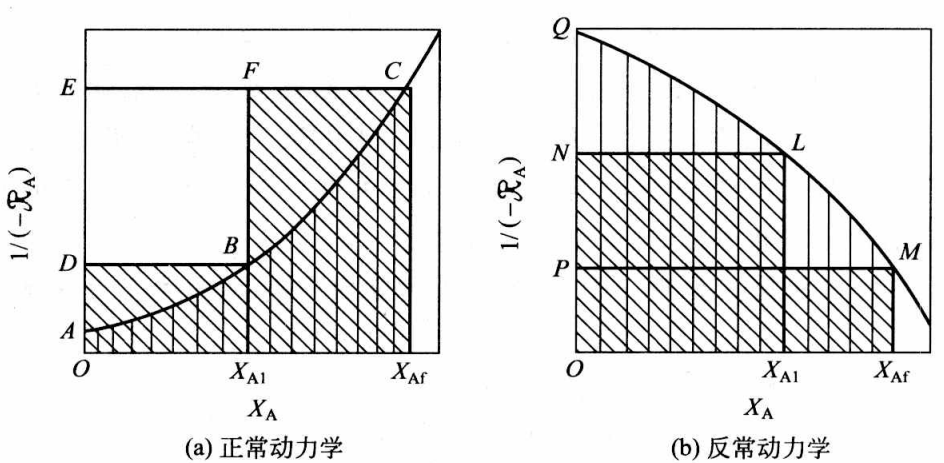
\includegraphics[width=.78\linewidth]{figs/fig4.3.png}
    \end{figure}

\end{frame}


\begin{frame}
    \frametitle{管式与釜式反应器反应体积的比较}

    自催化反应\ch{A -> P}，$r = kc_\mathrm{A}c_\mathrm{P}$：反应速率先增大后减小。

    ~\\
    \begin{minipage}{.48\linewidth}
        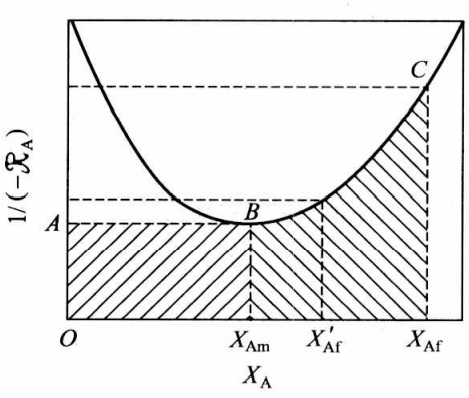
\includegraphics[width=\linewidth]{figs/fig4.4.png}
    \end{minipage}\hfill
    \begin{minipage}{.48\linewidth}
        \only<1>{
            \begin{question}
                \begin{enumerate}
                  \item 最终转化率小于$X_\mathrm{Am}$，管式与釜式反应器反应体积的比较？
                  \item 最终转化率大于$X_\mathrm{Am}$，管式与釜式反应器反应体积的比较？
                  \item 最终转化率大于$X_\mathrm{Am}$，如何选择反应器（可多个）使反应体积最小？
                \end{enumerate}
            \end{question}
        }
        \only<2>{
            \begin{enumerate}
            \item 若最终转化率小于$X_\mathrm{Am}$，$V_\text{管}>V_\text{釜}$
            \item 若最终转化率大于$X_\mathrm{Am}$，
            
            $V_\text{管}$可能大于也可能小于$V_\text{釜}$
            \item 最终转化率大于$X_\mathrm{Am}$情况下，最好的办法是采用两个反应器串联，先用釜式反应器使转化率达到$X_\mathrm{Am}$，再用管式反应器。
        \end{enumerate}
        }
    \end{minipage}

\end{frame}


\begin{frame}[t]
    \frametitle{}
    \begin{redblock}{借助大模型思考以下问题}
        自催化反应\ch{A -> P}，$r = kc_\mathrm{A}c_\mathrm{P}$，反应过程中总摩尔浓度守恒，当$c_\mathrm{A} = c_\mathrm{P}$时，反应速率最大。那么：
        \begin{enumerate}
          \item \ch{A -> 2 P}，$r = kc_\mathrm{A}c_\mathrm{P}$，什么时候反应速率最大？$(c_\mathrm{A0} = c_\mathrm{A0}, c_\mathrm{P0} = 0)$
          \item \ch{2 A -> P}，$r = kc_\mathrm{A}c_\mathrm{P}$，什么时候反应速率最大？$(c_\mathrm{A0} = c_\mathrm{A0},c_\mathrm{P0} = 0)$
          \item \ch{A -> P}，$r = kc_\mathrm{A}c_\mathrm{P}^2$，什么时候反应速率最大？$(c_\mathrm{A0} = c_\mathrm{A0}, c_\mathrm{P0} = 0)$
        \end{enumerate}
    \end{redblock}
\end{frame}


\begin{frame}
    \frametitle{管式与釜式反应器复合反应收率的比较}
    \begin{figure}
        \centering
        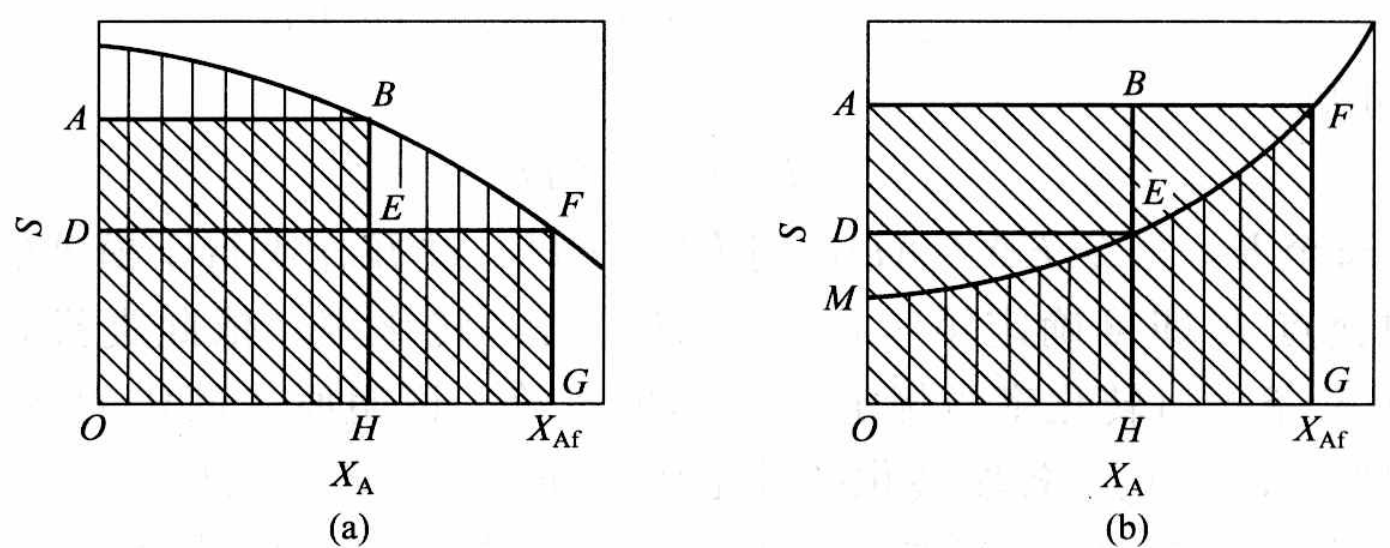
\includegraphics[width=.9\linewidth]{figs/fig3.9.png}
    \end{figure}
    间歇釜式反应器的性能与等容下的管式反应器相同。

    (a)管式反应器的最终收率大于连续釜式反应器。(b)反之。

\end{frame}


\begin{frame}
    \frametitle{管式反应器的加料方式}

    \begin{minipage}{0.42\linewidth}
        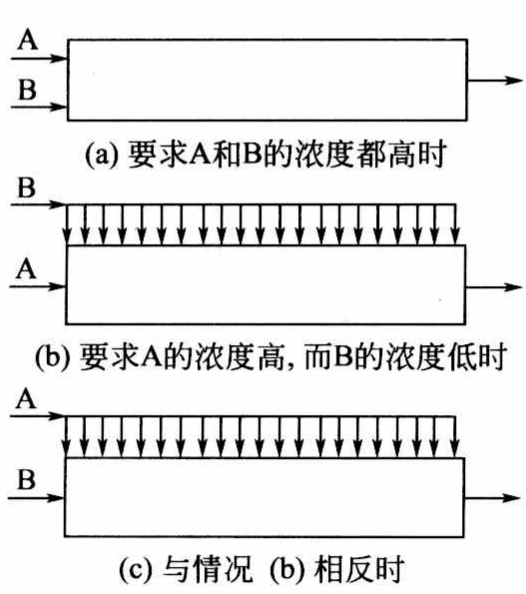
\includegraphics[width=\linewidth]{figs/fig4.5.png}
    \end{minipage}\hfill
    \begin{minipage}{0.56\linewidth}
        根据对反应物浓度的不同要求，可以对管式反应器采用不同的加料方式。
        \begin{itemize}
            \item[(a)] 当要求A和B的浓度都高时，可将两者同时在反应器的一端加入
            \item[(b)] 如要求A的浓度高，而B的浓度低，除了可以使进料中A大量过剩外，也可将A全部由反应器一端加入，而B则沿反应器的轴向分段加入。
            \item[(c)] 要求A的浓度低，B的浓度高时按图c加料。
        \end{itemize}
    \end{minipage}

\end{frame}


\begin{frame}[t]
    \frametitle{}

    \begin{block}{习题4.7}
        拟设计一等温反应器进行下列液相反应
        \[
            \ch{A + B -> R} \qquad r_\mathrm{R}=k_1c_\mathrm{A}c_\mathrm{B}
        \]
        \[
            \ch{2 A -> S} \qquad r_\mathrm{S} = k_2 c_\mathrm{A}^2
        \]
        目的产物是R，且R与B极难分离。试问

        (1) 在原料配比上有何要求？

        (2) 若采用活塞流反应器，应采用什么样的加料方式？

        (3) 如用半间歇反应器，又应用什么样的加料方式？
    \end{block}

\end{frame}


\begin{frame}[t]
    \frametitle{}

    \begin{question}
        习题4.14

        习题4.18
    \end{question}

\end{frame}



\section{循环反应器}


\begin{frame}[t]
    \frametitle{循环反应器}
    \begin{figure}
        \centering
        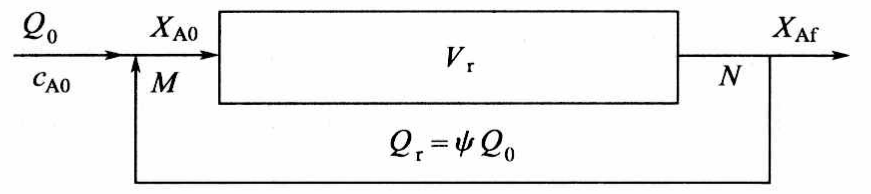
\includegraphics[width=.75\linewidth]{figs/fig4.6.png}
    \end{figure}
    \only<1>{
    \begin{itemize}
        \item 物料处理量$=?$
        \item 入口转化率$=?$
    \end{itemize}
    }
    \only<2>{
        反应器物料处理量
        \[
            Q_0 + Q_\mathrm{r} = (1 + \varphi) Q_0
        \]
        对M点作A的物料衡算
        \[
            Q_{0} c_{\mathrm{A} 0}+\varphi Q_{0} c_{\mathrm{A} 0}(1-X_{\mathrm{Af}})=(1+\varphi) Q_{0} c_{\mathrm{A} 0}(1-X_{\mathrm{A} 0})
        \]
        \[
            X_{\mathrm{A} 0}=\frac{\varphi  X_{\mathrm{Af}}}{1+\varphi}
        \]
    }
    \only<3>{
        \[
        V_{\mathrm{r}}=(1+\varphi) Q_{0} c_{\mathrm{A} 0} \int_{\frac{\varphi X_{\mathrm{Af}}}{1+\varphi}}^{X_{\mathrm{Af}}} \frac{\mathrm{d} X_{\mathrm{A}}}{(-\mathscr{R}_{\mathrm{A}})}
    \]
    \begin{itemize}
        \item 当$\varphi \to  0$时，$X_{\mathrm{A0}}=0$，$V_{\mathrm{r}}=Q_{0} c_{\mathrm{A} 0} \int_{0}^{X_{\mathrm{Af}}} \frac{\mathrm{d} X_{\mathrm{A}}}{(-\mathscr{R}_{\mathrm{A}})}$
        \item 当$\varphi \to \infty $时，$X_{\mathrm{A0}} \to X_{\mathrm{Af}}$，相当于恒定转化率$X_{\mathrm{Af}}$下操作的釜式反应器。
    \end{itemize}
    }
\end{frame}


\begin{frame}[t]
    \frametitle{}
    \begin{question}
        有一液相反应\ch{A -> P}，其速率方程为$r_\mathrm{A} = kc_\mathrm{A}$ \si{kmol/(m^3.min)}，反应温度下，$k=1$\si{min^{-1}}，$c_\mathrm{A0}=2$ \si{kmol/m^3}，每小时处理1000 mol原料A，要求最终转化率为90\%。
        
    （1）为使所需反应体积最小，采用何种型式反应器好？并算出所选用的反应体积。

    （2）如果采用循环反应器，当循环比$\phi = 2$时，反应体积为多少？

    （3）当循环比$\phi = \infty$时，反应体积为多少？

    （4）当循环比$\phi = 0$时，反应体积为多少？
    \end{question}
\end{frame}


\begin{frame}[t]
    \frametitle{}
    \begin{block}{习题4.22}
        有一自催化液相反应\ch{A -> P}，其速率方程为$r_\mathrm{A} = kc_\mathrm{A}c_\mathrm{p}$ \si{kmol/(m^3.min)}，反应温度下，$k=1$\si{m^3/(kmol.min)}，$c_\mathrm{A0}=2$ \si{kmol/m^3}，每小时处理1000 mol原料，其中A占99\%（摩尔分数），其余为P。要求最终转化率为90\%。
        
    （1）为使所需反应体积最小，采用何种型式反应器好？并算出所选用的反应体积。

    （2）如果采用循环反应器，请确定最佳循环比及反应体积。

    （3）当循环比$\phi = \infty$时，反应体积为多少？

    （4）当循环比$\phi = 0$时，反应体积为多少？
    \end{block}
\end{frame}


\section{变温管式反应器}


\begin{frame}
    \frametitle{变温管式反应器}

    工业反应器极少情况下是等温的，绝大多数都是在变温条件下操作。
    \begin{itemize}
        \item 化学反应过程都伴随着热效应，有些热效应还相当大，即使采用各种换热方式移走热量（放热反应）或者输入热量（吸热反应），对于工业反应器都难以维持等温。
        \item 许多反应过程等温操作的效果并不好，而要求有一最佳温度分布。如工业上进行合成氨，合成甲醇之类的可逆放热反应，便属于这种情况。
        \item 一些复杂反应、其主、副反应的活化能大小不同，温度的高低对主、副反应速率的影响也不同。所以，可通过改变温度的方法来改变产物的分布，使目的产物的收率最大。
    \end{itemize}

\end{frame}


\begin{frame}
    \frametitle{管式反应器的热量衡算式}

    取微元反应体积$\dif V_r$为控制体积作热量衡算

    若忽略动能和位能的变化而又不存在轴功时，对于等压过程
    \[
        \dif H = \dif q
    \]
    设反应流体的质量速度为$G$，管式反应器的直径为$d_\mathrm{t}$，则$\dif V_r = (\pi / 4) d_\mathrm{t}^2 \dif Z$

    若反应流体在微元反应体积中的温度变化为dT，定态下的焓变为
    \[
        \mathrm{d} H=[(-\mathscr{R}_{\mathrm{A}})(\Delta H_{\mathrm{r}})_{\mathrm{T}_{\mathrm{r}}} \mathrm{d} Z+G C_{\mathrm{pt}} \mathrm{d} T](\pi / 4) d_{\mathrm{t}}^{2}
    \]
    \[
        \mathrm{d} q=U(T_{\mathrm{C}}-T) \pi d_{\mathrm{t}} \mathrm{d} Z
    \]
    代入$\dif H = \dif q$，得到管式反应器的轴向温度分布方程
    \[
        G C_{\mathrm{pt}} \frac{\mathrm{d} T}{\mathrm{~d} Z}=(-\mathscr{R}_{\mathrm{A}})(-\Delta H_{\mathrm{r}})_{\mathrm{T}_{\mathrm{r}}}-4 U(T-T_{\mathrm{C}}) / d_{\mathrm{t}}
    \]

\end{frame}


\begin{frame}
    \frametitle{管式反应器的热量衡算式}

    将$Q_{0} c_{\mathrm{A} 0}=\frac{G(\pi d_{\mathrm{t}}^{2} / 4) w_{\mathrm{A} 0}}{M_{\mathrm{A}}} \text { 及 } \mathrm{d} V_{\mathrm{r}}=\frac{\pi}{4} d_{\mathrm{t}}^{2} \mathrm{~d} Z$代入管式反应器物料衡算方程得
    \[
        \frac{G w_{\mathrm{A} 0}}{M_{\mathrm{A}}} \frac{\mathrm{d} X_{\mathrm{A}}}{\mathrm{d} Z}=-\mathscr{R}_{\mathrm{A}}(X_{\mathrm{A}})
    \]
    代入管式反应器的轴向温度分布方程，得温度与转化率的关系式
    \[
        G C_{\mathrm{pt}} \frac{\mathrm{d} T}{\mathrm{~d} Z}=\frac{G w_{\mathrm{A} 0}(-\Delta H_{\mathrm{r}})_{\mathrm{T}_{\mathrm{r}}}}{M_{\mathrm{A}}} \frac{\mathrm{d} X_{\mathrm{A}}}{\mathrm{d} Z}-\frac{4 U}{d_{\mathrm{t}}}(T-T_{\mathrm{C}})
    \]

\end{frame}


\begin{frame}
    \frametitle{绝热管式反应器}

    若反应系在绝热条件下进行
    \[
        \mathrm{d} T=\frac{w_{\mathrm{A} 0}(-\Delta H_{\mathrm{r}})_{\mathrm{T}_{\mathrm{r}}}}{M_{\mathrm{A}}C_{\mathrm{pt}}} \mathrm{d} X_{\mathrm{A}}
    \]
    如不考虑热容随物料组成及温度而变，当入口处$T=T_0$，$X_\mathrm{A}=0$，且$T_\mathrm{r}=T_0$，积分上式得
    \[
        T - T_0 = \lambda X_\mathrm{A}
    \]
    \[
        \lambda = \frac{w_{\mathrm{A} 0}(-\Delta H_{\mathrm{r}})_{\mathrm{T}_{\mathrm{r}}}}{\bar C_{\mathrm{pt}}M_{\mathrm{A}}}
    \]
    \begin{itemize}
        \item 管式反应器，绝热方程式反映了不同轴向位置上转化率与温度的关系。
        \item 间歇反应器，反映了不同时间下转化率与温度的关系。
        \item 连续釜式反应器，反映了反应器出口转化率相对应的操作温度。
    \end{itemize}
    

\end{frame}


\begin{frame}
    \frametitle{绝热管式反应器}

    \begin{minipage}{.48\linewidth}
        \begin{figure}            
        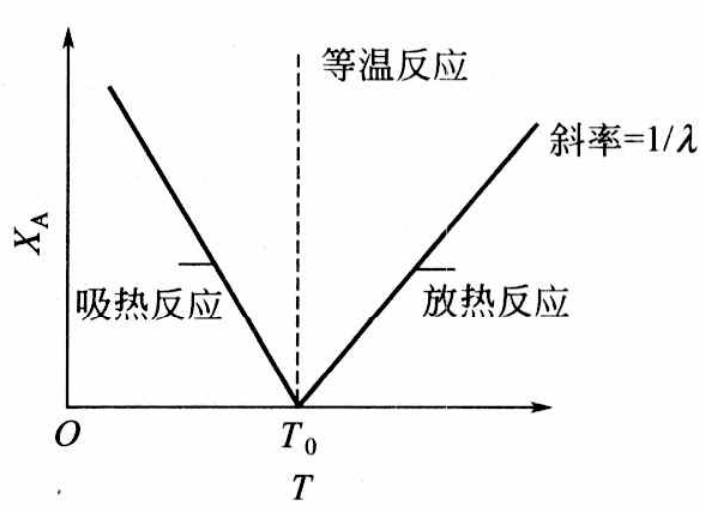
\includegraphics[width=\linewidth]{figs/fig4.7.png}
        \caption{绝热反应过程转化率与温度的关系}
        \end{figure}
    \end{minipage}\hfill
    \begin{minipage}{.48\linewidth}
        \begin{itemize}
            \item 该直线斜率为$1/\lambda$
            \item 放热反应，$\lambda>0$
            \item 吸热反应，$\lambda<0$
            \item 等温反应，$\lambda=0$
        \end{itemize}
    \end{minipage}

    \begin{itemize}
        \item 绝热条件下进行吸热反应时，反应温度随转化率的增加而下降
        \item 进行不可逆放热反应时，反应温度随转化率的增加而升高
    \end{itemize}

\end{frame}


\begin{frame}
    \frametitle{绝热管式反应器}

    \begin{minipage}{.48\linewidth}
        \begin{figure}            
        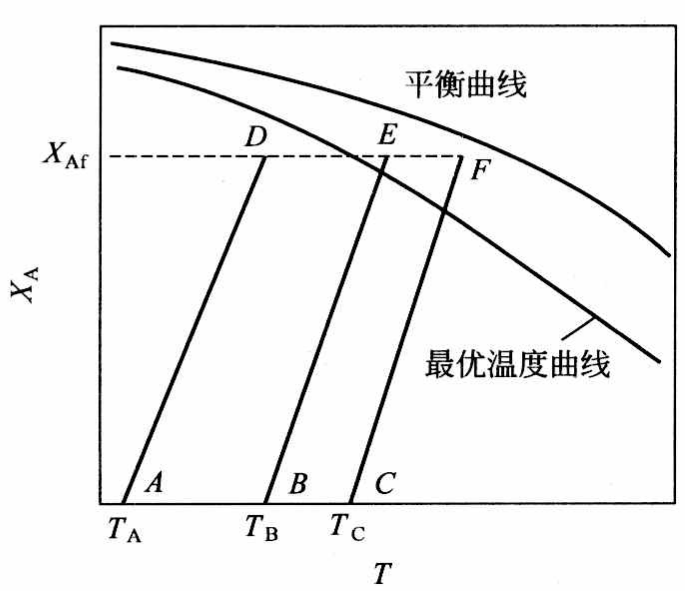
\includegraphics[width=\linewidth]{figs/fig4.8.png}
        \caption{可逆放热反应转化率与温度的关系}
        \end{figure}
    \end{minipage}\hfill
    \begin{minipage}{.48\linewidth}
        \begin{itemize}
            \item AD、BE、CF为不同进料温度下的绝热操作线。
            \item 对于一定的转化率，当反应温度低于最佳温度时，反应速率总是随温度的升高而增加，高于最佳温度时则随温度的升高而降低。
            \item 按BE线操作，其平均反应速率要大于AD线操作。
            \item 按CF线操作并不见得比BE线好，因为反应后期太接近平衡了，所以存在一最佳的进料温度。
        \end{itemize}
    \end{minipage}

\end{frame}


\begin{frame}
    \frametitle{绝热管式反应器的最佳的进料温度}

    \begin{minipage}{.35\linewidth}
        \begin{figure}            
        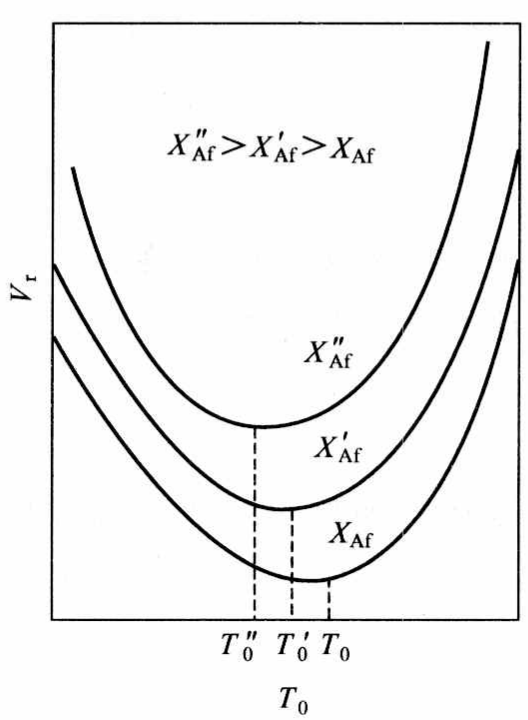
\includegraphics[width=\linewidth]{figs/fig4.9.png}
        \end{figure}
    \end{minipage}\hfill
    \begin{minipage}{.63\linewidth}
        \begin{itemize}
            \item 图中每条曲线是对一定的最终转化率而作出的
            \item 最终转化率越高，则最佳进料温度越低
            \item $X_\mathrm{AF}''>X_\mathrm{AF}'>X_\mathrm{AF}$，相应的最佳进料温度$T_0''<T_0'<T_0$
        \end{itemize}
    \end{minipage}

\end{frame}


\begin{frame}[t]
    \frametitle{}
    \vspace{-0.5em}
    \begin{block}{例4.7}
        在内径为1.22 m的绝热管式反应器中进行乙苯催化脱氢反应。进料温度为898K，其余数据和要求同例4.5。反应速率常数和温度的关系为
        \[
            k = 3.452\times 10^{-5}\exp (-10983/T) \quad \mathrm{kmol/(s\cdot kg \cdot Pa)}
        \]
        不同温度下的化学平衡常数值可根据下列近似式估算
        \[
            K = 3.96\times 10^{11}\exp (-14520/T) \quad \mathrm{Pa}
        \]
        反应混合物的平均比热容为\SI{2.177}{kJ.(kg.K)}，反应热等于\SI{1.39e5}{J/mol}。催化剂床层的堆密度为\SI{1440}{kg/m^3}。试计算：

        (1) 催化剂用量；(2) 反应器的轴向温度及转化率分布。
        \tcblower
        \pause
        \vspace{-1em}
        \footnotesize
        \[
            \frac{\mathrm{d} X_{\mathrm{A}}}{\mathrm{d} Z}=\frac{4.104 \times 10^{6}}{21+X_{\mathrm{A}}} \exp \left(-\frac{10983}{898-137 X_{\mathrm{A}}}\right) \times\left[1-X_{\mathrm{A}}-\frac{3.03 \times 10^{-7} X_{\mathrm{A}}^{2}}{21+X_{\mathrm{A}}} \exp \left(\frac{14520}{898-137 X_{\mathrm{A}}}\right)\right] 
        \]
    \end{block}
\end{frame}


\begin{frame}
    \frametitle{}
    \begin{figure}[htpb]
        \centering
        
\includegraphics[width=\linewidth]{例4.7}
    \end{figure}
\end{frame}


\begin{frame}
    \frametitle{非绝热变温管式反应器}

    某些情况下，不适宜采用绝热操作
    \begin{itemize}
        \item 热效应很大的化学反应，绝热操作会使进出口物料温差太大
        \item 可逆放热反应，反应温度沿轴向升高，温度升高则平衡转化率降低，应用绝热反应器就得不到较高的转化率
        \item 可逆吸热反应，反应温度沿轴向降低，反应速率越来越慢
        \item 不可逆吸热反应，反应温度沿轴向降低，反应速率越来越慢，平衡转化率还会下降
        \item 由于某些原因，反应温度一定要控制在一定范围内的反应
            \begin{itemize}
                \item[\bullet] 温度过高会爆炸
                \item[\bullet] 温度过高会损坏催化剂
            \end{itemize}
    \end{itemize}
    这些情况下，在化学反应进行的同时必须与环境进行热交换

\end{frame}


\begin{frame}
    \frametitle{换热介质}

    常用高温换热介质
    \begin{itemize}
        \item 燃烧液体或气体燃料产生的烟道气
        \item 熔盐
        \item 高压蒸汽
    \end{itemize}
    常用低温换热介质
    \begin{itemize}
        \item 水
        \item 空气
        \item 反应原料
    \end{itemize}

\end{frame}


\begin{frame}
    \frametitle{列管式反应器}
    \begin{minipage}{0.68\linewidth}
        提高传热面积可采用列管式反应器，即将许多直径较小的管式反应器并联操作。
        \begin{enumerate}
          \item 提高传热面积
          \item 避免径向温差过大
        \end{enumerate}
        设计多管并联反应器时，一般可认为各管情况相同，所以只对一根管考察即能反应整个反应器的工况。
    \end{minipage}\hfill
    \begin{minipage}{0.28\linewidth}
        \begin{figure}[htpb]
            \centering
            
\includegraphics[width=\linewidth]{列管式反应器}
        \end{figure}
    \end{minipage}
    
\end{frame}


\begin{frame}[t]
    \frametitle{}
    \begin{block}{例4.8}
        采用144根直径为0.101 m的反应管并联操作，以代替例4.7中直径为1.22 m的绝热管式反应器进行乙苯催化脱氢反应。这些反应管外用温度恒定为1100 K的烟道气加热，烟道气与反应管内反应气体间的总传热系数为\SI{2.85}{W/(m^2.K)}。其他条件和要求同例4.7，试计算反应器的轴向转化率及温度分布，以及乙苯转化率达60\%时所需的催化剂量。
    \end{block}
\end{frame}


\begin{frame}
    \frametitle{}
    \begin{figure}[htpb]
        \centering
        
\includegraphics[width=\linewidth]{例4.8}
    \end{figure}
\end{frame}


\section{管式反应器的最佳温度序列}


\begin{frame}[t]
    \frametitle{单一反应}
    单一反应，以生产强度最大为目标
    \only<1>{        
    \begin{table}[]
        \begin{tabular}{
            >{\columncolor[HTML]{f4f8f9}}c 
    >{\columncolor[HTML]{f4f8f9}}c 
    >{\columncolor[HTML]{f4f8f9}}c }
        \hline
        & 等温 & 变温 \\ \hline
        不可逆反应 &  &  \\
        可逆吸热反应 &  &  \\
        可逆放热反应 & \phantom{高温操作有利$^{[1]}$} & \phantom{按最佳温度操作序列，先高后低$^{[3]}$} \\ \hline
        \end{tabular}
        \end{table}
    }
    \only<2>{
        \begin{table}[]
            \begin{tabular}{
                >{\columncolor[HTML]{f4f8f9}}c 
        >{\columncolor[HTML]{f4f8f9}}c 
        >{\columncolor[HTML]{f4f8f9}}c }
            \hline
             & 等温 & 变温 \\ \hline
            不可逆反应 & 高温操作有利$^{[1]}$ & 先低后高$^{[2]}$ \\
            可逆吸热反应 & 高温操作有利$^{[1]}$ & 先低后高$^{[2]}$ \\
            可逆放热反应 & 存在最佳温度~~~~ & 按最佳温度操作序列，先高后低$^{[3]}$ \\ \hline
            \end{tabular}
            \end{table}
        
            \begin{itemize}
                \item[{[1]}] 实际上能够采用多高的操作温度，还受到反应器的构成材料、能源、催化剂的耐热性能等方面的限制，需要结合这些因素来考虑。
                \item[{[2]}] 反应过程中，由于反应物浓度逐渐降低而导致反应速率下降，如果保持反应过程的温度逐渐上升，则可补偿由于浓度降低而引起的反应速率减小。
                \item[{[3]}] 要完全按最佳温度曲线操作，实行起来会困难不少，但应力图接近。
            \end{itemize}
    }

\end{frame}


\begin{frame}[t]
    \frametitle{}
    \begin{question}
        如下平行反应，$E_1<E_2$，如何选择最佳温度策略
        \[
        \ch{A + B ->[1] P}
        \]
        \[
            \ch{A + B ->[2] Q}
        \]
        \begin{enumerate}
            \item 以目标产物收率最大为目标
            \item 以生产强度最大为目标
        \end{enumerate}
    \end{question}
\end{frame}


\begin{frame}[t]
    \frametitle{}
    \begin{question}
        如下平行反应，$E_1<E_2$，如何选择最佳温度策略
        \[
        \ch{A + B ->[1] P}
        \]
        \[
            \ch{A + B ->[2] Q}
        \]
        \tcblower
        \begin{enumerate}
            \item 以目标产物收率最大为目标
            
            应在较低温度下操作，以减少Q的生成。
            \item 以生产强度最大为目标
            
            应先低温后高温。低温有利于P的生成，反应后期浓度下降反应速率降低，采用高温提高反应速率。但副产物Q的量会增加。
        \end{enumerate}
    \end{question}
\end{frame}


\begin{frame}[t]
    \frametitle{复合反应}

    复合反应，以目标产物收率最大为目标
\only<1>{
    \begin{table}[]\
        \begin{tabular}{
        >{\columncolor[HTML]{f4f8f9}}c |
        >{\columncolor[HTML]{f4f8f9}}c 
        >{\columncolor[HTML]{f4f8f9}}c }
        \hline
        \cellcolor[HTML]{f4f8f9}                   & $E_1 < E_2$ &  \\ \cline{2-3} 
        \multirow{-2}{*}{\cellcolor[HTML]{f4f8f9} \makecell{\ch{A + B -> P} \\ \ch{A + B -> Q}}} & $E_1 > E_2$ &   \\ \hline
        \cellcolor[HTML]{f4f8f9}                   & $E_1 < E_2$ & \makecell{等温操作：\phantom{温度越低越好~~~~} \\ 变温操作：\phantom{先高温后低温$^{[2]}$}} \\ \cline{2-3} 
        \multirow{-2}{*}{\cellcolor[HTML]{f4f8f9} \ch{A -> P -> Q}} & $E_1 > E_2$ & 等温操作：\phantom{温度越低越好~~~~} \\ \hline
        \end{tabular}
        \end{table}
}
\only<2>{
    \begin{table}[]\
        \begin{tabular}{
        >{\columncolor[HTML]{f4f8f9}}c |
        >{\columncolor[HTML]{f4f8f9}}c 
        >{\columncolor[HTML]{f4f8f9}}c }
        \hline
        \cellcolor[HTML]{f4f8f9}                   & $E_1 < E_2$ & 低温操作有利$^{[1]}$ \\ \cline{2-3} 
        \multirow{-2}{*}{\cellcolor[HTML]{f4f8f9} \makecell{\ch{A + B -> P} \\ \ch{A + B -> Q}}} & $E_1 > E_2$ & 高温操作有利 ~~~~  \\ \hline
        \cellcolor[HTML]{f4f8f9}                   & $E_1 < E_2$ & \makecell{等温操作：温度越低越好~~~~ \\ 变温操作：先高温后低温$^{[2]}$} \\ \cline{2-3} 
        \multirow{-2}{*}{\cellcolor[HTML]{f4f8f9} \ch{A -> P -> Q}} & $E_1 > E_2$ & 等温操作：温度越高越好~~~~ \\ \hline
        \end{tabular}
        \end{table}
    
        \begin{itemize}
            \item[{[1]}] 总选择性提高，但生产强度下降，所需的反应体积增大。
            \item[{[2]}] 先高温是为了加快第一个反应，促使P的生成，待P累积到一定的量后，降低温度以减小副产物Q的生成。
        \end{itemize}
}
\end{frame}



\begin{frame}
    \frametitle{化学反应工程问题优化}

    \begin{center}
        \begin{tikzpicture}
            \node (A) at (0,0) {A + B};
            \node (B) at (2,0) {Q};
            \node (C) at (4,0) {P};
            \node (D) at (0,-2) {X};
            \node (E) at (2,-2) {Y};
            \draw[->] (A) -- (B) node[above,midway]{1};
            \draw[->] (B) -- (C) node[above,midway]{3};
            \draw[->] (A) -- (D) node[right,midway]{2};
            \draw[->] (B) -- (E) node[right,midway]{4};
            \end{tikzpicture}
    \end{center}
    
    设P为目的产物，且$E_1 < E_2$，$E_3 > E_4$。
    \begin{itemize}
        \item 由于$E_1 < E_2$，低温有利于生成Q而不利于生成X
        \item 由于$E_3 > E_4$，低温有利于Q转化成Y而不利于转化成P
        \item 采用等温操作无论选定什么温度，P的收率都不会高
        \item 只有保持由低到高的温度序列，才能获得较高的P的收率
    \end{itemize}
\end{frame}


\begin{frame}
    \frametitle{化学反应工程问题优化}

    \begin{center}
        \begin{tikzpicture}
            \node (A) at (0,0) {A + B};
            \node (B) at (2,0) {Q};
            \node (C) at (4,0) {P};
            \node (D) at (0,-2) {X};
            \node (E) at (2,-2) {Y};
            \draw[->] (A) -- (B) node[above,midway]{1};
            \draw[->] (B) -- (C) node[above,midway]{3};
            \draw[->] (A) -- (D) node[right,midway]{2};
            \draw[->] (B) -- (E) node[right,midway]{4};
            \end{tikzpicture}
    \end{center}

    设P为目的产物。
    \begin{itemize}
        \item 若$E_1 > E_2$，$E_3 > E_4$
        \item 若$E_1 < E_2$，$E_3 < E_4$
        \item 若$E_1 > E_2$，$E_3 < E_4$
        \item 若$E_1 < E_2$，$E_3 > E_4$
    \end{itemize}
\end{frame}


\begin{frame}
    \frametitle{化学反应工程问题优化}

    \begin{center}
        \begin{tikzpicture}
            \node (A) at (0,0) {A + B};
            \node (B) at (2,0) {Q};
            \node (C) at (4,0) {P};
            \node (D) at (0,-2) {X};
            \node (E) at (2,-2) {Y};
            \draw[->] (A) -- (B) node[above,midway]{1};
            \draw[->] (B) -- (C) node[above,midway]{3};
            \draw[->] (A) -- (D) node[right,midway]{2};
            \draw[->] (B) -- (E) node[right,midway]{4};
            \end{tikzpicture}
    \end{center}

    设P为目的产物。
    \begin{itemize}
        \item 若$E_1 > E_2$，$E_3 > E_4$，高温操作
        \item 若$E_1 < E_2$，$E_3 < E_4$，低温操作
        \item 若$E_1 > E_2$，$E_3 < E_4$，由高温到低温
        \item 若$E_1 < E_2$，$E_3 > E_4$，由低温到高温
    \end{itemize}
\end{frame}


\begin{frame}[t]
    \frametitle{}
    \begin{block}{管式反应器设计案例分析}
        设计工业规模的管式反应器，由纯乙烷进料裂解生产乙烯，计划年产量14万吨。设计条件：

        （1）原料为纯乙烷，\ch{C2H6 -> C2H4 + H2}，反应为一级不可逆反应；

        （2）反应条件等温1100K，恒压600 kPa，转化率80\%；

        （3）反应活化能为343.7 kJ/mol，1000K时，速率常数$k = 0.0725 \ \mathrm{s^{-1}}$；

        （4）一年工作时间按300天。
    \end{block}
\end{frame}


\begin{frame}[t]
    \frametitle{}
    \begin{block}{釜式反应器设计案例分析}
        某化工厂拟设计一台间歇釜生产乙酸丁酯，计划年产量720t。

        设计条件：

        （1）原料采用乙酸和丁醇
        \[
            \ch{CH3COOH(A) + C4H9OH(B) -> CH3COOC4H9(R) + H2O(S)}
        \]
        （2）反应条件恒温，373K，少量硫酸作催化剂，转化率50\%；

        （3）动力学方程：$r_\mathrm{A} = kc_\mathrm{A}^2$，速率常数$k=0.0174$ \si{m^3.kmol^{-1}.min^{-1}}，反应活化能为45.4 kJ/mol；

        （4）进料摩尔比：乙酸：丁醇$=1:4.97$，原料液密度$\rho = 750$ \si{kg.m^3}（假设反应前后不变）；

        （5）一年工作时间按300天，辅助时间为0.5 h；

        （6）反应器装填系数为0.7。
    \end{block}
\end{frame}


\end{document}